\documentclass[11pt,a4paper]{report}    % chapters, a title page and an abstract, on A4

% References
\usepackage{csquotes}                   % quotation marks that follow the document's language
\usepackage[backend=biber,style=apa,natbib=true]{biblatex} % APA 7; compile with Biber
\DeclareLanguageMapping{australian}{british-apa}
\usepackage{xurl} % allow long bibliography URLs to wrap within the page
\addbibresource{references.bib}

% Page
\usepackage[margin=25mm]{geometry}      % 25 mm margins all round
\usepackage{parskip}                    % a blank line between paragraphs instead of an indent
\usepackage[australian]{babel}          % Australian hyphenation, and \today as 17 October 2026
\usepackage{iftex}                      % tells which TeX engine is running
\ifPDFTeX                               % for pdfLaTeX only:
  \usepackage[T1]{fontenc}              % proper accented letters, and text that copies cleanly from the PDF
  \usepackage{lmodern}                  % Latin Modern, a crisp scalable version of the default font
\fi                                     % XeLaTeX, LuaLaTeX and Tectonic already use Unicode fonts, which print a typed ’ or é as it is
\usepackage{microtype}                  % small spacing tweaks so lines break more evenly

% Maths
\usepackage{amsmath}                    % align, cases, matrices and \text inside maths
\usepackage{amssymb}                    % extra symbols such as \mathbb{R}

% Figures and tables
\usepackage{graphicx}                   % \includegraphics, for photos and saved plots
\usepackage{booktabs}                   % \toprule, \midrule and \bottomrule for clean tables
\usepackage{siunitx}                    % numbers and units: \qty{6.6}{\kilo\watt}, aligned table columns
\sisetup{group-separator={,},group-minimum-digits=4} % 7,790 with a comma, as Australian style has it
\usepackage{pgfplots}                   % charts drawn from data, right in the document
\pgfplotsset{compat=1.18}               % use current pgfplots behaviour (label placement and so on)

% Links
\usepackage[hidelinks]{hyperref}        % clickable contents, cross-references and citations, without coloured boxes
\hypersetup{                            % details shown in the PDF viewer’s document properties
  pdftitle  = {Rooftop solar output across a Melbourne year},
  pdfauthor = {Your Name},
  pdflang   = {en-AU}
}
\usepackage[capitalise,noabbrev]{cleveref} % \cref{fig:monthly} writes “Figure 4.1” for you; load after hyperref

\begin{document}

% The title page is numbered a, so its link target can’t clash with page 1 or page i
\pagenumbering{alph}
\begin{titlepage}
  \centering
  \vspace*{30mm}
  {\LARGE\bfseries Rooftop solar output across a Melbourne year\par}
  \vspace{12mm}
  {\Large Your Name\par}
  \vspace{25mm}
  A thesis submitted in partial fulfilment of the requirements for the degree of\par
  \vspace{3mm}
  {\large Bachelor of Engineering (Honours)\par}
  \vfill
  School of Engineering\par
  Your University\par
  \vspace{6mm}
  October 2026
\end{titlepage}

% Front matter is numbered i, ii, iii; chapter 1 starts again at 1
\pagenumbering{roman}

\chapter*{Abstract}
A typical \qty{6.6}{\kilo\watt} rooftop system in suburban Melbourne was logged every five minutes for a year.
It produced \qty{7790}{\kilo\watt\hour}, three times as much in December as in June. Output
followed the sun's height more closely than the weather: cloudy summer days still beat clear
winter ones. A simple model built from panel area, efficiency and temperature predicts the
monthly totals to within 6 per cent, which is close enough to size a system before it is
bought.

\chapter*{Acknowledgements}
Thanks to my supervisor for their patience, and to the household that let a data logger live
in their meter box for a year.

\tableofcontents
\listoffigures
\listoftables

\clearpage
\pagenumbering{arabic}

% Long chapters can live in their own files: \include{chapters/introduction}
\chapter{Introduction}\label{ch:intro}

One in three Australian houses now has solar panels on the roof, yet most owners only see a
quarterly bill. This thesis asks a simple question: how much does a typical system produce
in each month of the year, and can that be predicted before it is installed?

\cref{ch:background} sets out the physics of a photovoltaic panel, \cref{ch:method}
describes the system and how it was measured, \cref{ch:results} presents a year of data, and
\cref{ch:conclusion} draws the threads together.

\chapter{Background}\label{ch:background}

A panel turns a fraction of the sunlight that falls on it into electricity
\citep{Masters2013}. To a first approximation the power it delivers is
\begin{equation}\label{eq:power}
  P = \eta \, A \, G,
\end{equation}
where $\eta$ is the panel's efficiency, $A$ its area and $G$ the irradiance on its surface.
Efficiency drops as the panel heats up, which \citet{Duffie2013} model as a straight line,
\begin{equation}\label{eq:temperature}
  \eta = \eta_{\text{ref}} \bigl[ 1 - \beta \, (T_c - T_{\text{ref}}) \bigr],
\end{equation}
with $\beta \approx \qty{0.004}{\per\kelvin}$ for crystalline silicon. On a hot January
afternoon a roof-mounted panel can reach \qty{65}{\degreeCelsius}, costing it about
16 per cent of its rated output.

\chapter{Method}\label{ch:method}

The system faces north at a pitch of \ang{22.5}, the most common roof angle in the area.
\cref{tab:system} lists its main parts. A logger on the inverter recorded power every five
minutes from 1 January to 31 December 2025.

\begin{table}[ht]
  \centering
  \caption{The system that was measured.}\label{tab:system}
  \begin{tabular}{l r}
    \toprule
    Part             & Value                         \\
    \midrule
    Panels           & 18 $\times$ \qty{370}{\watt}   \\
    Panel area       & \qty{35.1}{\metre\squared}     \\
    Rated efficiency & \qty{19.0}{\percent}          \\
    Inverter         & \qty{5.0}{\kilo\watt}          \\
    \bottomrule
  \end{tabular}
\end{table}

\chapter{Results}\label{ch:results}

\cref{fig:monthly} shows the energy produced in each month. Output peaks in December and
January and bottoms out in June, when the sun is low and days are short.

\begin{figure}[ht]
  \centering
  % a saved image works too: \includegraphics[width=0.8\textwidth]{monthly.png}
  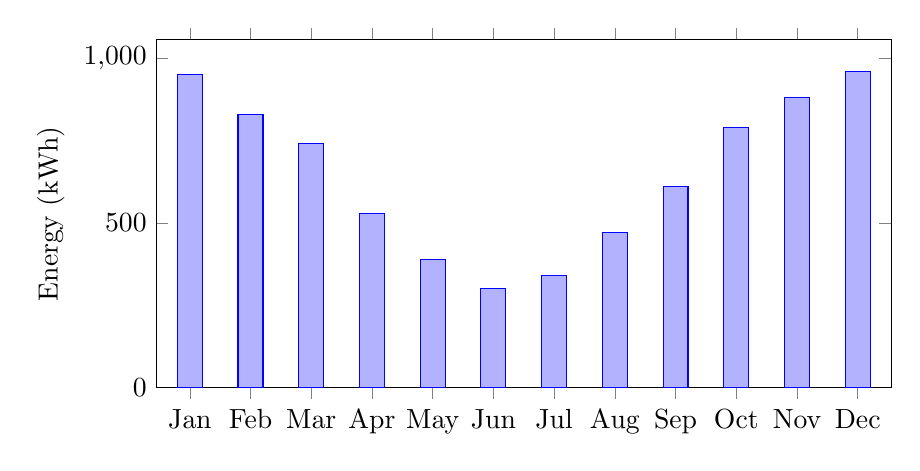
\begin{tikzpicture}
    \begin{axis}[
        ybar, bar width=9pt, width=0.9\textwidth, height=60mm,
        ymin=0, ylabel={Energy (kWh)},
        symbolic x coords={Jan,Feb,Mar,Apr,May,Jun,Jul,Aug,Sep,Oct,Nov,Dec},
        xtick=data, enlarge x limits=0.05,
      ]
      \addplot coordinates {(Jan,950) (Feb,830) (Mar,740) (Apr,530) (May,390) (Jun,300)
                            (Jul,340) (Aug,470) (Sep,610) (Oct,790) (Nov,880) (Dec,960)};
    \end{axis}
  \end{tikzpicture}
  \caption{Energy produced in each month of 2025.}\label{fig:monthly}
\end{figure}

Grouping the months by season (\cref{tab:seasons}) makes the pattern plainer: summer
produces about two and a half times as much as winter. Using \cref{eq:power,eq:temperature} with
monthly irradiance and temperature gives totals within 6 per cent of those measured.

\begin{table}[ht]
  \centering
  \caption{Energy by season, measured and modelled.}\label{tab:seasons}
  \begin{tabular}{l S[table-format=4.0] S[table-format=4.0] S[table-format=-1.1]}
    \toprule
    Season & {Measured (kWh)} & {Modelled (kWh)} & {Difference (\%)} \\
    \midrule
    Summer & 2740 & 2810 & 2.6  \\
    Autumn & 1660 & 1580 & -4.8 \\
    Winter & 1110 & 1050 & -5.4 \\
    Spring & 2280 & 2350 & 3.1  \\
    \midrule
    Year   & 7790 & 7790 & 0.0  \\
    \bottomrule
  \end{tabular}
\end{table}

\chapter{Conclusion}\label{ch:conclusion}

A year of five-minute readings shows that a north-facing \qty{6.6}{\kilo\watt} system in Melbourne produces
about \qty{7.8}{\mega\watt\hour} a year, most of it between October and March. The simple
model of \cref{ch:background} is good enough to size a system, and \citet{Lamport1994} made
writing it up rather less painful.

% The bibliography comes from references.bib; it shows only the entries you cite
\cleardoublepage
\phantomsection
\addcontentsline{toc}{chapter}{Bibliography}

\printbibliography

\appendix
\chapter{Logger settings}\label{app:logger}

The logger sampled the inverter's output every \qty{5}{\minute} and stored the readings as
comma-separated values, one file per day.

\end{document}
